\scanpage{139}
\figure{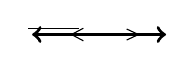
\begin{tikzpicture}\draw[<->,very thick](0,0)--(1.7,0);\draw(-.05,.08)--(.6,.08);\draw(.65,.08)--(.5,0)--(.65,-.08);\draw(1.2,.07)--(1.35,0)--(1.2,-.07);\end{tikzpicture}}
\margin{deg ext}
\diagram{\begin{tikzcd}[column sep=large,row sep=large]
 A_n^0\simeq k\{\{T\}\}\{\{X_0,\ldots,X_n\}\}/(\sum X_i-T)_{pd}\arrow[d,equal]
 &k\{\{T\}\}\{\{X_0,\ldots,X_n\}\}\arrow[l,two heads,tail,"{\text{épi}}"']\arrow[d,equal]\\
 k\{\{X_0,\ldots,X_n\}\}
 &k\{\{T,X_0,\ldots,X_n\}\}\arrow[l,two heads,tail,"{\substack{X_i\mapsfrom X_i\\\sum_{0\leq i\leq n}X_i\mapsfrom T}}"']
\end{tikzcd}}
\deleted{\figure{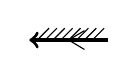
\begin{tikzpicture}\draw[<-,very thick](0,0)--(1,0);\draw(.7,.12)--(.5,0)--(.7,-.12);\foreach\x in{.1,.2,.3,.4,.5,.6,.7,.8}{\draw(\x,0)--(\x+.15,.15);}\end{tikzpicture}}}
\unsure{duals}
\diagram{\begin{tikzcd}[column sep=large,row sep=large]
 (A^n)_0\simeq k[U+Y_0,U+Y_1,\ldots,U+Y_n]\arrow[d,equal]
 &k[U][Y_0,\ldots,Y_n]\arrow[d,equal]\\
 k[Z_0,Z_1,\ldots,Z_n]\arrow[r,tail,"{Z_i\mapsto U+Y_i}"']
 &k[U,Y_0,\ldots,Y_n]
 \arrow[from=1-1,to=1-2,tail,"{\text{mono}}"]
\end{tikzcd}}
\margin{deg ext}
\margin{[l'image est \unsure{l'intersection} des noyaux des \unsure{op. diff.}
$\left(\frac{\partial}{\partial Y_0}+\cdots+\frac{\partial}{\partial Y_n}-\frac{\partial}{\partial U}\right)^{(i)}$]}
\figure{\begin{tikzpicture}\draw(0,1.5)..controls(.4,1)and(1.1,.5)..(1.6,.2);\draw(1.65,.2)--(2.3,.18);\end{tikzpicture}}
\[
\begin{aligned}
\langle X_0^{(i_0)}\cdots X_n^{(i_n)},Z_0^{j_0}\cdots Z_n^{j_n}\rangle
 &=\prod_{0\leq\alpha\leq n}\delta_{i_\alpha,j_\alpha}\\
 &=\begin{cases}0&\text{si }(i_\alpha)\ne(j_\alpha)\\1&\text{si }(i_\alpha)=(j_\alpha)\end{cases}
\end{aligned}
\]
\[
\begin{aligned}
\langle T^{(\lambda)}X_0^{(i_0)}\cdots X_n^{(i_n)},U^\mu Y_0^{j_0}\cdots Y_n^{j_n}\rangle
 &=\delta_{\lambda,\mu}\unsure{\delta_{(i_\alpha)(j_\alpha)}}\\
 &=\begin{cases}0&\text{si }(\lambda,(i_\alpha))\ne(\mu,(j_\alpha))\\1&\text{si }\text{---}=\text{---}\end{cases}
\end{aligned}
\]

\margin{degré tot = deg ext\quad i.e. \unsure{deg compl.}$=0$}
\diagram{\begin{tikzcd}[column sep=large]
 A_n^{*=*}\simeq\bigwedge_k^*[dX_0,\ldots,dX_n]/(\sum dX_i)
 &\bigwedge_k^*[dX_0,\ldots,dX_n]\arrow[l,two heads,tail,"{\text{épi}}"']
\end{tikzcd}}
\unsure{duals}
\diagram{\begin{tikzcd}[row sep=large,column sep=large]
 (A^n)_{*=*}\simeq(\bigwedge_k^*[y_0,\ldots,y_n])^{\unsure{!|'}}\arrow[r,tail]\arrow[d,equal]
 &\bigwedge_k^*[y_0,\ldots,y_n]\\
 \bigwedge_k^*\bigl(\underbrace{[y_0,\ldots,y_n]^{\unsure{!|'}}}_{\substack{\text{ss-e.v. de}\\ky_0\oplus\cdots\oplus ky_n\\\text{formé aux vect. dont la}\\\text{somme des coord.}=0}}\bigr)&
\end{tikzcd}}
\margin{l'image est le noyau de $i_X$, où $X$ est la forme sur $ky_0\oplus\cdots\oplus ky_n$ ``somme des coordonnées'' et où $i_X$ est le prod. int.}

\uline{NB} On a un isom can
\[
\bigwedge_k^{\deleted{\unsure{*}}\unsure{n-1|n}}([y_0\ldots y_n]^{\unsure{'|!}})
\simeq\bigwedge_k^n([y_0,\ldots,y_n])\simeq k
\]
déduit de la suite exacte
\diagram{\begin{tikzcd}[column sep=small]
0\arrow[r,dash]&{[y_0,\ldots,y_n]'}\arrow[r,dash]&{[y_0,\ldots,y_n]}\arrow[r,dash]&k\arrow[r,dash]&0
\end{tikzcd}}
Donc
\[
 (A^n)_n\overset{\text{iso can}}\simeq(A^n)_0\simeq k[Z_0,\ldots,Z_n]
\]
\margin{deg ext}
\figure{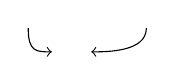
\begin{tikzpicture}\draw[->](0,.3)..controls(0,0)and(.1,0)..(.3,0);\draw[->](1.5,.3)..controls(1.5,0)and(1,0)..(.8,0);\end{tikzpicture}}
d'où
\[
\unsure{\kappa_n}:k[U]\longrightarrow k[Z_0,\ldots,Z_n]
\]
\margin{138}
